%%%%%%%%%%%%%%%%%%%%%%%%%%%%%%%%%%%%%%%%%%%%%%%%%%%%%%%%%%%%%%%%%%%%%%%%%%%%%%%%%%
\begin{frame}[fragile]\frametitle{}

\begin{center}
{\Large Topic Modeling using Gensim}
\end{center}
\end{frame}


%%%%%%%%%%%%%%%%%%%%%%%%%%%%%%%%%%%%%%%%%%%%%%%%%%%%%%%%%%%%%%%%%%%%%%%%%%%%%%%%%%
\begin{frame}[fragile]\frametitle{Recap LDA via Matrix}
  \begin{itemize}
\item In vector space, any corpus (collection of documents) can be represented as a document-term matrix. 
\item The following matrix shows a corpus of N documents D1, D2, D3 \ldots Dn and vocabulary size of M words W1,W2 \ldots Wn. 
\item The value of i,j cell gives the frequency count of word Wj in Document Di.
  \end{itemize}

\begin{center}
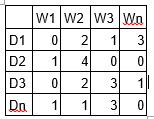
\includegraphics[width=0.5\linewidth,keepaspectratio]{top7}
\end{center}

\end{frame}

%%%%%%%%%%%%%%%%%%%%%%%%%%%%%%%%%%%%%%%%%%%%%%%%%%%%%%%%%%%%%%%%%%%%%%%%%%%%%%%%%%
\begin{frame}[fragile]\frametitle{Recap LDA via Matrix}
  \begin{itemize}
\item LDA converts this Document-Term Matrix into two lower dimensional matrices - M1 and M2.
\item  M1 is a document-topics matrix and M2 is a topic - terms matrix with dimensions (N,  K) and (K, M) respectively, 
\item Where N is the number of documents, K is the number of topics and M is the vocabulary size.
  \end{itemize}

\begin{center}
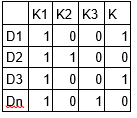
\includegraphics[width=0.45\linewidth,keepaspectratio]{top8}
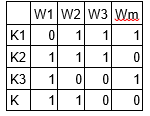
\includegraphics[width=0.5\linewidth,keepaspectratio]{top9}
\end{center}
\end{frame}

%%%%%%%%%%%%%%%%%%%%%%%%%%%%%%%%%%%%%%%%%%%%%%%%%%%%%%%%%%%%%%%%%%%%%%%%%%%%%%%%%%%
%\begin{frame}[fragile]\frametitle{Understand LDA via Matrix}
%  \begin{itemize}
%  	\item It Iterates through each word ``w'' for each document ``d'' and tries to adjust the current topic - word assignment with a new assignment. A new topic ``k'' is assigned to word ``w'' with a probability P which is a product of two probabilities $P_1$ and $P_2$.
%	\item For every topic, two probabilities $P_1$ and $P_2$ are calculated. $P_1 = P(topic_t / document_d)$ is the proportion of words in document d that are currently assigned to topic t. $P_2 = P(word_w / topic_t)$ is the proportion of assignments to topic t over all documents that come from this word w.
%  \end{itemize}
%\end{frame}
%
%
%%%%%%%%%%%%%%%%%%%%%%%%%%%%%%%%%%%%%%%%%%%%%%%%%%%%%%%%%%%%%%%%%%%%%%%%%%%%%%%%%%%
%\begin{frame}[fragile]\frametitle{Understand LDA via Matrix}
%  \begin{itemize}
%\item The current topic - word assignment is updated with a new topic with the probability, product of  $P_1$ and $P_1$ . 
%\item In this step, the model assumes that all the existing word - topic assignments except the current word are correct. 
%\item This is essentially the probability that $topic_t$ generated $word_w$, so it makes sense to adjust the current word's topic with new probability.
%\item After a number of iterations, a steady state is achieved where the document topic and topic term distributions are fairly good. This is the convergence point of LDA.
%  \end{itemize}
%\end{frame}


%%%%%%%%%%%%%%%%%%%%%%%%%%%%%%%%%%%%%%%%%%%%%%%%%%%%%%%%%%%%%%%%%%%%%%%%%%%%%%%%%%
\begin{frame}[fragile]\frametitle{Parameters of LDA}
  \begin{itemize}
\item Alpha represents document-topic density. More alpha more topics per document and vice versa.
\item Beta represents topic-word density. More beta more words per topic and vice versa.
\item Number of Topics - Number of topics to be extracted from the corpus. Optimal number of topics by using Kullback Leibler Divergence Score.
\item Number of Topic Terms - Number of terms composed in a single topic. A low number is recommended.
  \end{itemize}
\end{frame}
%%%%%%%%%%%%%%%%%%%%%%%%%%%%%%%%%%%%%%%%%%%%%%%%%%%%%%%%%%%%%%%%%%%%%%%%%%%%%%%%%%
\begin{frame}[fragile]\frametitle{What is Gensim?}
  \begin{itemize}
  	\item Gensim is a free Python framework for doing topic modelling.
	\item Installation: \lstinline|pip install gensim|

	\begin{lstlisting}
import gensim
>>>  help(gensim)
\end{lstlisting}
  	\item We can transform corpora from one vector space to another using models. 
	\item Transformations can bring out hidden structure in the corpus, such as revealing relationships between words and documents. 
	\item They can also represent the corpus in a more compact way, preserving much information while consuming fewer resources.
	\item A gensim 'transformation' is any object which accepts a sparse document via dictionary notation and returns another sparse document.''
		  \end{itemize}
\end{frame}

%%%%%%%%%%%%%%%%%%%%%%%%%%%%%%%%%%%%%%%%%%%%%%%%%%%%%%%%%%%%%%%%%%%%%%%%%%%%%%%%%%
\begin{frame}[fragile]\frametitle{Preparing Corpus}
  \begin{itemize}
  	\item Start by turning a large set of documents into numeric vectors. 
	\item A document can be as short as one word, or as long as many pages of text, or anywhere in between.
	\item A sentence or a tweet can be a document.
	\item In gensim, a corpus is an iterable that returns its documents as sparse vectors (one-hot like).
	\item How you generate those vectors from the documents is up to you?
	\item If your features are the presence or absence of words, your corpus is in what's called ''bucket of words'' (BOW) format. 			
	\item Gensim provides a convenience class called TextCorpus for creating a such corpus from a text file.

  \end{itemize}
\end{frame}

%%%%%%%%%%%%%%%%%%%%%%%%%%%%%%%%%%%%%%%%%%%%%%%%%%%%%%%%%%%%%%%%%%%%%%%%%%%%%%%%%%
\begin{frame}[fragile]\frametitle{Preparing Corpus}
	\begin{lstlisting}
texts = [" ".join(file.readlines()[1:]) for file in files]
tokenised = [[word.lower() for word in WordPunctTokenizer().tokenize(text) if word.lower() not in stopwords]]
dictionary = corpora.Dictionary(tokenised)
corpus = [dictionary.doc2bow(text) for text in tokenised]
corpora.MmCorpus.serialize('./corpus.mm', corpus)

for word in corpus[0]:
	print dictionary.id2token[word[0]],word[1]
\end{lstlisting}
\end{frame}



%%%%%%%%%%%%%%%%%%%%%%%%%%%%%%%%%%%%%%%%%%%%%%%%%%%%%%%%%%%%%%%%%%%%%%%%%%%%%%%%%%
\begin{frame}[fragile]\frametitle{Vectorization}
  \begin{itemize}
  	\item For BOW, we also need a dictionary
	\item Dictionary maps feature ids back to features (words). 
	\item So the vectors indicate the presence of words in particular documents, and the resulting matrix containing these vectors will represent all the words appearing in all the documents. 
  \end{itemize}
\begin{lstlisting}
>>> corpus = TextCorpus(file_like_object)
>>> print corpus.dictionary
Dictionary(8472 unique tokens)
\end{lstlisting}
\end{frame}


%%%%%%%%%%%%%%%%%%%%%%%%%%%%%%%%%%%%%%%%%%%%%%%%%%%%%%%%%%%%%%%%%%%%%%%%%%%%%%%%%%
\begin{frame}[fragile]\frametitle{Vectorization}
  \begin{itemize}
\item One useful transformation that we can generate from our BOW corpus is term frequency/inverse document frequency (TFIDF). 
\item Instead of a count of word appearances in a document, we get a score for each word that also takes into account the global frequency of that word. 
\item So a word's TFIDF value in a given document increases proportionally to the number of times a word appears in that particular document, but is offset by the frequency of the word in the entire corpus, which helps to control for the fact that some words are generally more common than others.
  \end{itemize}
\end{frame}

%%%%%%%%%%%%%%%%%%%%%%%%%%%%%%%%%%%%%%%%%%%%%%%%%%%%%%%%%%%%%%%%%%%%%%%%%%%%%%%%%%
\begin{frame}[fragile]\frametitle{Vectorization}
\begin{lstlisting}
>>> tfidf_trans = models.TfidfModel(wiki_corpus, id2word=dictionary)  
>>> tfidf_trans[documents]  
[[(40, 0.23), (6, 0.12), (78, 0.65)], [(39, ...]

\end{lstlisting}
  \begin{itemize}
\item The wiki\_corpus TFIDF space as (word\_id, word\_weight) tuples where weight is a positive, normalized float. 
\item These documents can be anything, new and unseen, as long as they have been tokenized and put into the BOW representation using the same tokenizer and dictionary $word \rightarrow id$ mappings that were used for the wiki corpus.
  \end{itemize}
\end{frame}
%
%%%%%%%%%%%%%%%%%%%%%%%%%%%%%%%%%%%%%%%%%%%%%%%%%%%%%%%%%%%%%%%%%%%%%%%%%%%%%%%%%%%
%\begin{frame}[fragile]\frametitle{Vectorization}
%\begin{lstlisting}
%>>> lsi_trans = models.LsiModel(corpus=tfidf_corpus, id2word=dictionary, num_features=400)  
%\end{lstlisting}
%  \begin{itemize}
%\item TFIDF corpus itself is not all that interesting except as a stepping stone to another model called LSI. 
%\item Latent semantic indexing/analysis (LSI/LSA) - grandaddy of topic modelling similarity techniques. 
%  \end{itemize}
%\end{frame}

%%%%%%%%%%%%%%%%%%%%%%%%%%%%%%%%%%%%%%%%%%%%%%%%%%%%%%%%%%%%%%%%%%%%%%%%%%%%%%%%%%
\begin{frame}[fragile]\frametitle{Gensim Models}
Let's now run the LDA algorithm, which actually takes only one line. 
\begin{lstlisting}
lda = gensim.models.ldamodel.LdaModel(corpus=corpus, id2word=dictionary, num_topics=5)
lda.show_topics(topics=-1)
\end{lstlisting}
\end{frame}

%%%%%%%%%%%%%%%%%%%%%%%%%%%%%%%%%%%%%%%%%%%%%%%%%%%%%%%%%%%%%%%%%%%%%%%%%%%%%%%%%%
\begin{frame}[fragile]\frametitle{Example of LDA: Preparing Documents}
Here are the sample documents combining together to form a corpus.
\begin{lstlisting}
doc1 = "Sugar is bad to consume. My sister likes to have sugar, but not my father."
doc2 = "My father spends a lot of time driving my sister around to dance practice."
doc3 = "Doctors suggest that driving may cause increased stress and blood pressure."
doc4 = "Sometimes I feel pressure to perform well at school, but my father never seems to drive my sister to do better."
doc5 = "Health experts say that Sugar is not good for your lifestyle."

# compile documents
doc_complete = [doc1, doc2, doc3, doc4, doc5]
\end{lstlisting}
\end{frame}


%%%%%%%%%%%%%%%%%%%%%%%%%%%%%%%%%%%%%%%%%%%%%%%%%%%%%%%%%%%%%%%%%%%%%%%%%%%%%%%%%%
\begin{frame}[fragile]\frametitle{Example of LDA: Cleaning and Preprocessing}
We will remove the punctuations, stopwords and normalize the corpus.
\begin{lstlisting}
from nltk.corpus import stopwords
from nltk.stem.wordnet import WordNetLemmatizer
import string
stop = set(stopwords.words('english'))
exclude = set(string.punctuation)
lemma = WordNetLemmatizer()
def clean(doc):
    stop_free = " ".join([i for i in doc.lower().split() if i not in stop])
    punc_free = ''.join(ch for ch in stop_free if ch not in exclude)
    normalized = " ".join(lemma.lemmatize(word) for word in punc_free.split())
    return normalized

doc_clean = [clean(doc).split() for doc in doc_complete] 
\end{lstlisting}
\end{frame}

%%%%%%%%%%%%%%%%%%%%%%%%%%%%%%%%%%%%%%%%%%%%%%%%%%%%%%%%%%%%%%%%%%%%%%%%%%%%%%%%%%
\begin{frame}[fragile]\frametitle{Example of LDA: Preparing Document-Term Matrix}
To run any mathematical model on text corpus, it is a good practice to convert it into a matrix representation. LDA model looks for repeating term patterns in the entire DT matrix.
\begin{lstlisting}
# Importing Gensim
import gensim
from gensim import corpora

# Creating the term dictionary of our courpus, where every unique term is assigned an index. dictionary = corpora.Dictionary(doc_clean)

# Converting list of documents (corpus) into Document Term Matrix using dictionary prepared above.
doc_term_matrix = [dictionary.doc2bow(doc) for doc in doc_clean]
\end{lstlisting}
\end{frame}

%%%%%%%%%%%%%%%%%%%%%%%%%%%%%%%%%%%%%%%%%%%%%%%%%%%%%%%%%%%%%%%%%%%%%%%%%%%%%%%%%%
\begin{frame}[fragile]\frametitle{Example of LDA: Running LDA Model}
Next step is to create an object for LDA model and train it on Document-Term matrix.
\begin{lstlisting}
# Creating the object for LDA model using gensim library
Lda = gensim.models.ldamodel.LdaModel

# Running and Trainign LDA model on the document term matrix.
ldamodel = Lda(doc_term_matrix, num_topics=3, id2word = dictionary, passes=50)
\end{lstlisting}
\end{frame}


%%%%%%%%%%%%%%%%%%%%%%%%%%%%%%%%%%%%%%%%%%%%%%%%%%%%%%%%%%%%%%%%%%%%%%%%%%%%%%%%%%
\begin{frame}[fragile]\frametitle{Example of LDA: Results}
Next step is to create an object for LDA model and train it on Document-Term matrix.
\begin{lstlisting}
print(ldamodel.print_topics(num_topics=3, num_words=3))
['0.168*health + 0.083*sugar + 0.072*bad,
'0.061*consume + 0.050*drive + 0.050*sister,
'0.049*pressur + 0.049*father + 0.049*sister]
\end{lstlisting}
\end{frame}

%%%%%%%%%%%%%%%%%%%%%%%%%%%%%%%%%%%%%%%%%%%%%%%%%%%%%%%%%%%%%%%%%%%%%%%%%%%%%%%%%%
\begin{frame}[fragile]\frametitle{Tips to improve results of topic modeling}
  \begin{itemize}
\item The results of topic models are completely dependent on the features (terms) present in the corpus. 
\item The corpus is represented as document term matrix, which in general is very sparse in nature. 
\item Reducing the dimensionality of the matrix can improve the results of topic modelling. 
\item Frequency Filter: get rid of all those weak features ie low frequency words.
\item Part of Speech Tag Filter: Only NN* can be kept.
\item Add to stopwords (domain specific)
\item Batch Wise LDA: a corpus can be divided into batches of fixed sizes. Running LDA multiple times on these batches will provide different results, however, the best topic terms will be the intersection of all batches.
  \end{itemize}
\end{frame}
